\documentclass[letterpaper]{article}

\title{Project 01}
\date{April 20, 2016}
\author{David Durkin, Matt Reilly}

\usepackage{graphicx}
\usepackage{hyperref}
\usepackage[margin=1in]{geometry}

\begin{document}

\maketitle

This document provides an overview of our Project 01

\section*{Summary}

In this project we created a simple client named thor and a simple server called spidey. Then, we tested the interaction between the two, specifically measuring the latency and the throughput.

\section*{Latency}

In order to measure the average latency of spidey, we first added an option to thor called avg (-a) that, when enacted, would suppress everything except for the average time it takes per request. Then, we created a shell script called latency which runs the thor client 50 times in a row with 10 requests and the -a flag enacted, in the shell script associated files are filled with these time measures. We first ran the script on a spidey without forking enabled. Following this we calculated the averages of all those numbers and using a script named average, and loaded those values into a text file named single We then executed the same process on a spidey server with forking enabled and loaded those results into a text file called fork. Here are our results:

\begin{figure}[h!]
\centering
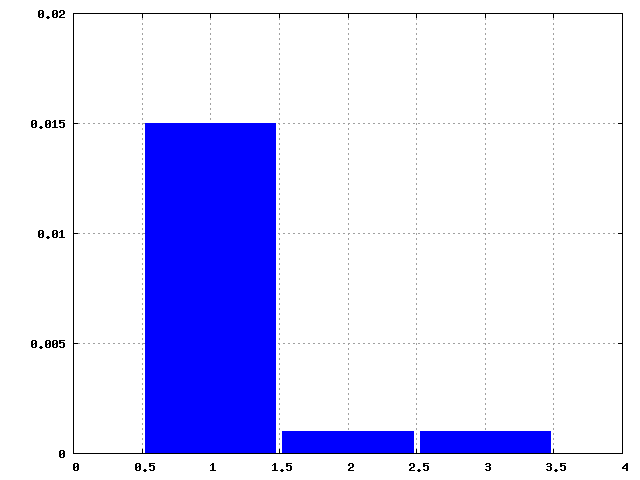
\includegraphics[width=4in]{single.png}
\caption{SINGLE CONNECION: From Left to Right: Directory Listings, Static Files, CGI Scrips (Time measured in seconds)}
\label{fig:Plot}
\end{figure}

\begin{figure}[h!]
\centering
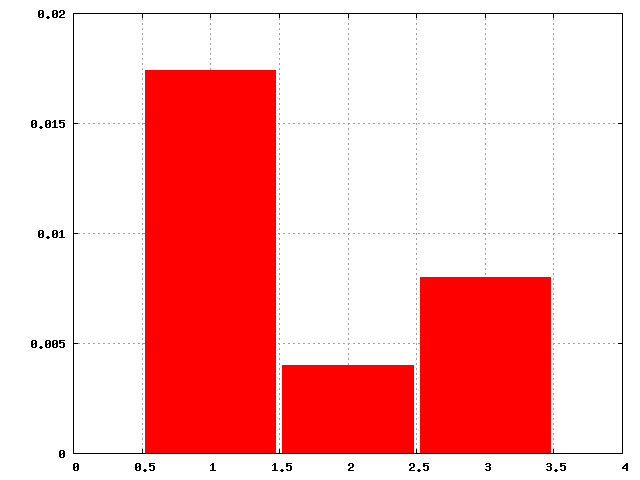
\includegraphics[width=4in]{fork.png}
\caption{FORK MODE: From Left to Right: Directory Listings, Static Files, CGI Scrips (Time measured in seconds)}
\label{fig:Plot}
\end{figure}

\section*{Throughput}

In order to measure the average throughput of spidey, we wrote a test_throughput shell script. This script has thor.py retrieve a small, medium, and large file. I then used awk to average the times.

Times with forking were always longer. There was a big jump in time from small to medium, and large was basically impossible.

\begin{figure}[h!]
\centering
\includegraphics[width=4in]{throughput.png}
\caption{Throughput while forking}
\label{fig:PLOT}
\end{figure}

\section*{Analysis}

Long story short: Forking takes time. It involves copying everything involved with execution (files, register states, RAM). As you can imagine, this takes time and resources, in turn slowing processes down. That is the chief downside of forking. 

Spidey also slowed down considerably with large files.

\section*{Comclusions}

This project taught us basic networking with python. Thor.py was out client, and spidey.py was our server. Our client sent a HTTP request, and the server responded to that request.  Implementing forming made the scripts way more complicated. Handling errors and file types also made spidey more complicated. Basic networking is a very important thing to know, so we're glad this project exposed us to it.

\end{document}